% Figura Anexo III: la equivalencia ricardiana: tres formas de financiar el mismo gasto conducen al mismo consumo
\documentclass[tikz,border=3pt]{standalone}
\usepackage[T1]{fontenc}
\usepackage[utf8]{inputenc}
\usepackage{amsmath}
\usetikzlibrary{arrows.meta,calc,positioning,shapes.misc}
\begin{document}
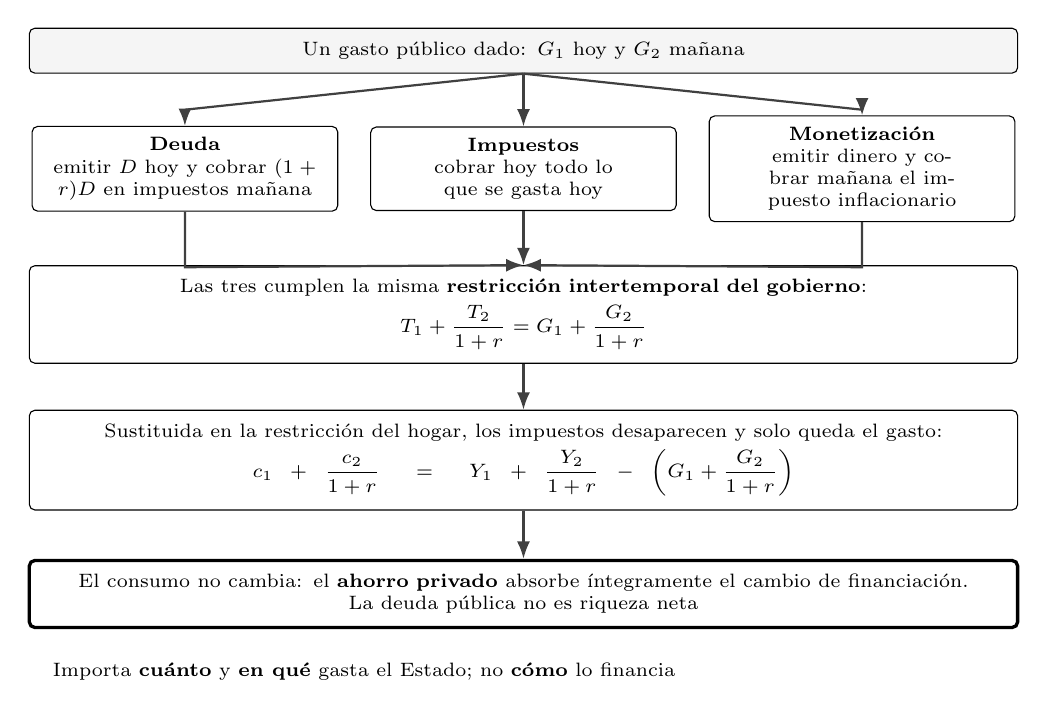
\begin{tikzpicture}[>={Latex[length=2.2mm]}, font=\footnotesize, node distance=0pt,
  caja/.style={draw, rounded corners=2pt, align=center, inner sep=4pt, text width=3.6cm, font=\scriptsize},
  ancha/.style={draw, rounded corners=2pt, align=center, inner sep=5pt, text width=12.2cm, font=\scriptsize},
  final/.style={draw, very thick, rounded corners=2pt, align=center, inner sep=5pt, text width=12.2cm, font=\scriptsize},
  fl/.style={->, thick, gray!50!black}]
  \node[ancha, fill=gray!8] (g) at (0,0) {Un gasto público dado: $G_1$ hoy y $G_2$ mañana};
  \node[caja] (deuda) at (-4.3,-1.5) {\textbf{Deuda}\\emitir $D$ hoy y cobrar $(1+r)D$ en impuestos mañana};
  \node[caja] (imp) at (0,-1.5) {\textbf{Impuestos}\\cobrar hoy todo lo que se gasta hoy};
  \node[caja] (mon) at (4.3,-1.5) {\textbf{Monetización}\\emitir dinero y cobrar mañana el impuesto inflacionario};
  \draw[fl] (g.south) -- (-4.3,-0.75) -- (deuda.north);
  \draw[fl] (g.south) -- (imp.north);
  \draw[fl] (g.south) -- (4.3,-0.75) -- (mon.north);
  \node[ancha] (rpi) at (0,-3.35) {Las tres cumplen la misma \textbf{restricción intertemporal del gobierno}:\\[2pt]\mbox{$T_1+\dfrac{T_2}{1+r}=G_1+\dfrac{G_2}{1+r}$}};
  \draw[fl] (deuda.south) -- (-4.3,-2.75) -- (rpi.north);
  \draw[fl] (imp.south) -- (rpi.north);
  \draw[fl] (mon.south) -- (4.3,-2.75) -- (rpi.north);
  \node[ancha] (hogar) at (0,-5.2) {Sustituida en la restricción del hogar, los impuestos desaparecen y solo queda el gasto:\\[2pt]$c_1+\dfrac{c_2}{1+r}=Y_1+\dfrac{Y_2}{1+r}-\left(G_1+\dfrac{G_2}{1+r}\right)$};
  \draw[fl] (rpi.south) -- (hogar.north);
  \node[final] (fin) at (0,-6.9) {El consumo no cambia: el \textbf{ahorro privado} absorbe íntegramente el cambio de financiación.\\La deuda pública no es riqueza neta};
  \draw[fl] (hogar.south) -- (fin.north);
  \node[align=left, anchor=north west, font=\scriptsize] at (-6.1,-7.65) {Importa \textbf{cuánto} y \textbf{en qué} gasta el Estado; no \textbf{cómo} lo financia};
\end{tikzpicture}
\end{document}
